\documentclass[12pt]{article}

% PACKAGES
\usepackage[utf8]{inputenc}
\usepackage[spanish]{babel} 
\usepackage[hidelinks]{hyperref}
\usepackage[margin = 1in]{geometry}
\usepackage{amssymb,amsmath,amsthm,amsfonts}
\usepackage{framed}
\usepackage{enumerate}
\usepackage{multicol}
\usepackage{graphicx}
\usepackage{parskip}
\usepackage{float}
\usepackage{cancel}
\usepackage{cellspace}
\usepackage{fancyhdr}
\usepackage{listings}
% \usepackage{titlesec}

% SETTINGS
\newcommand{\doublerule}[1][.4pt]{\noindent\makebox[0pt][l]{\rule[.7ex]{\linewidth}{#1}}\rule[.1ex]{\linewidth}{#1}}
\renewcommand{\qedsymbol}{\rule{0.7em}{0.7em}}
\addto\captionsspanish{\renewcommand{\contentsname}{Índice}}
\newcolumntype{M}[1]{>{\centering\arraybackslash}m{#1}}
\newenvironment{solution}{\begin{proof}[Solución]}{\end{proof}}
\graphicspath{{./img/}}
\decimalpoint

% HEAD AND FOOT
% \setlength{\headheight}{25pt}
% \setlength{\footskip}{25pt}
% \pagestyle{fancy}
% \renewcommand{\footrulewidth}{0.4pt}
% \fancyhf{}
% \fancypagestyle{empty}{
%     \fancyhf{}
% }

% REPORT OR BOOK
% \titleformat{\chapter}{\normalfont\huge}{\thechapter.}{20pt}{\huge \bf}
% \titlespacing{\chapter}{0pt}{0pt}{1cm}

% THEOREMS
\newtheorem*{observation}{Observación}
\newtheorem*{definition}{Definición}
\newtheorem*{theorem}{Teorema}
\newtheorem*{example}{Ejemplo}
\newtheorem*{lemma}{Lema}

% DATA
\title{Práctica Uno}
\author{Edzon Alanis}
\date{\today}
\newcommand{\signature}{Materia}
\newcommand{\professor}{Profesor}
\newcommand{\titlepagelogo}{./img/logo.png}

% SET VARIABLES
\makeatletter
\let\thetitle\@title
\let\theauthor\@author
\let\thedate\@date
\makeatother

\begin{document}
\maketitle
\section{Código (Python)}
\begin{figure}[H]
    \centering
    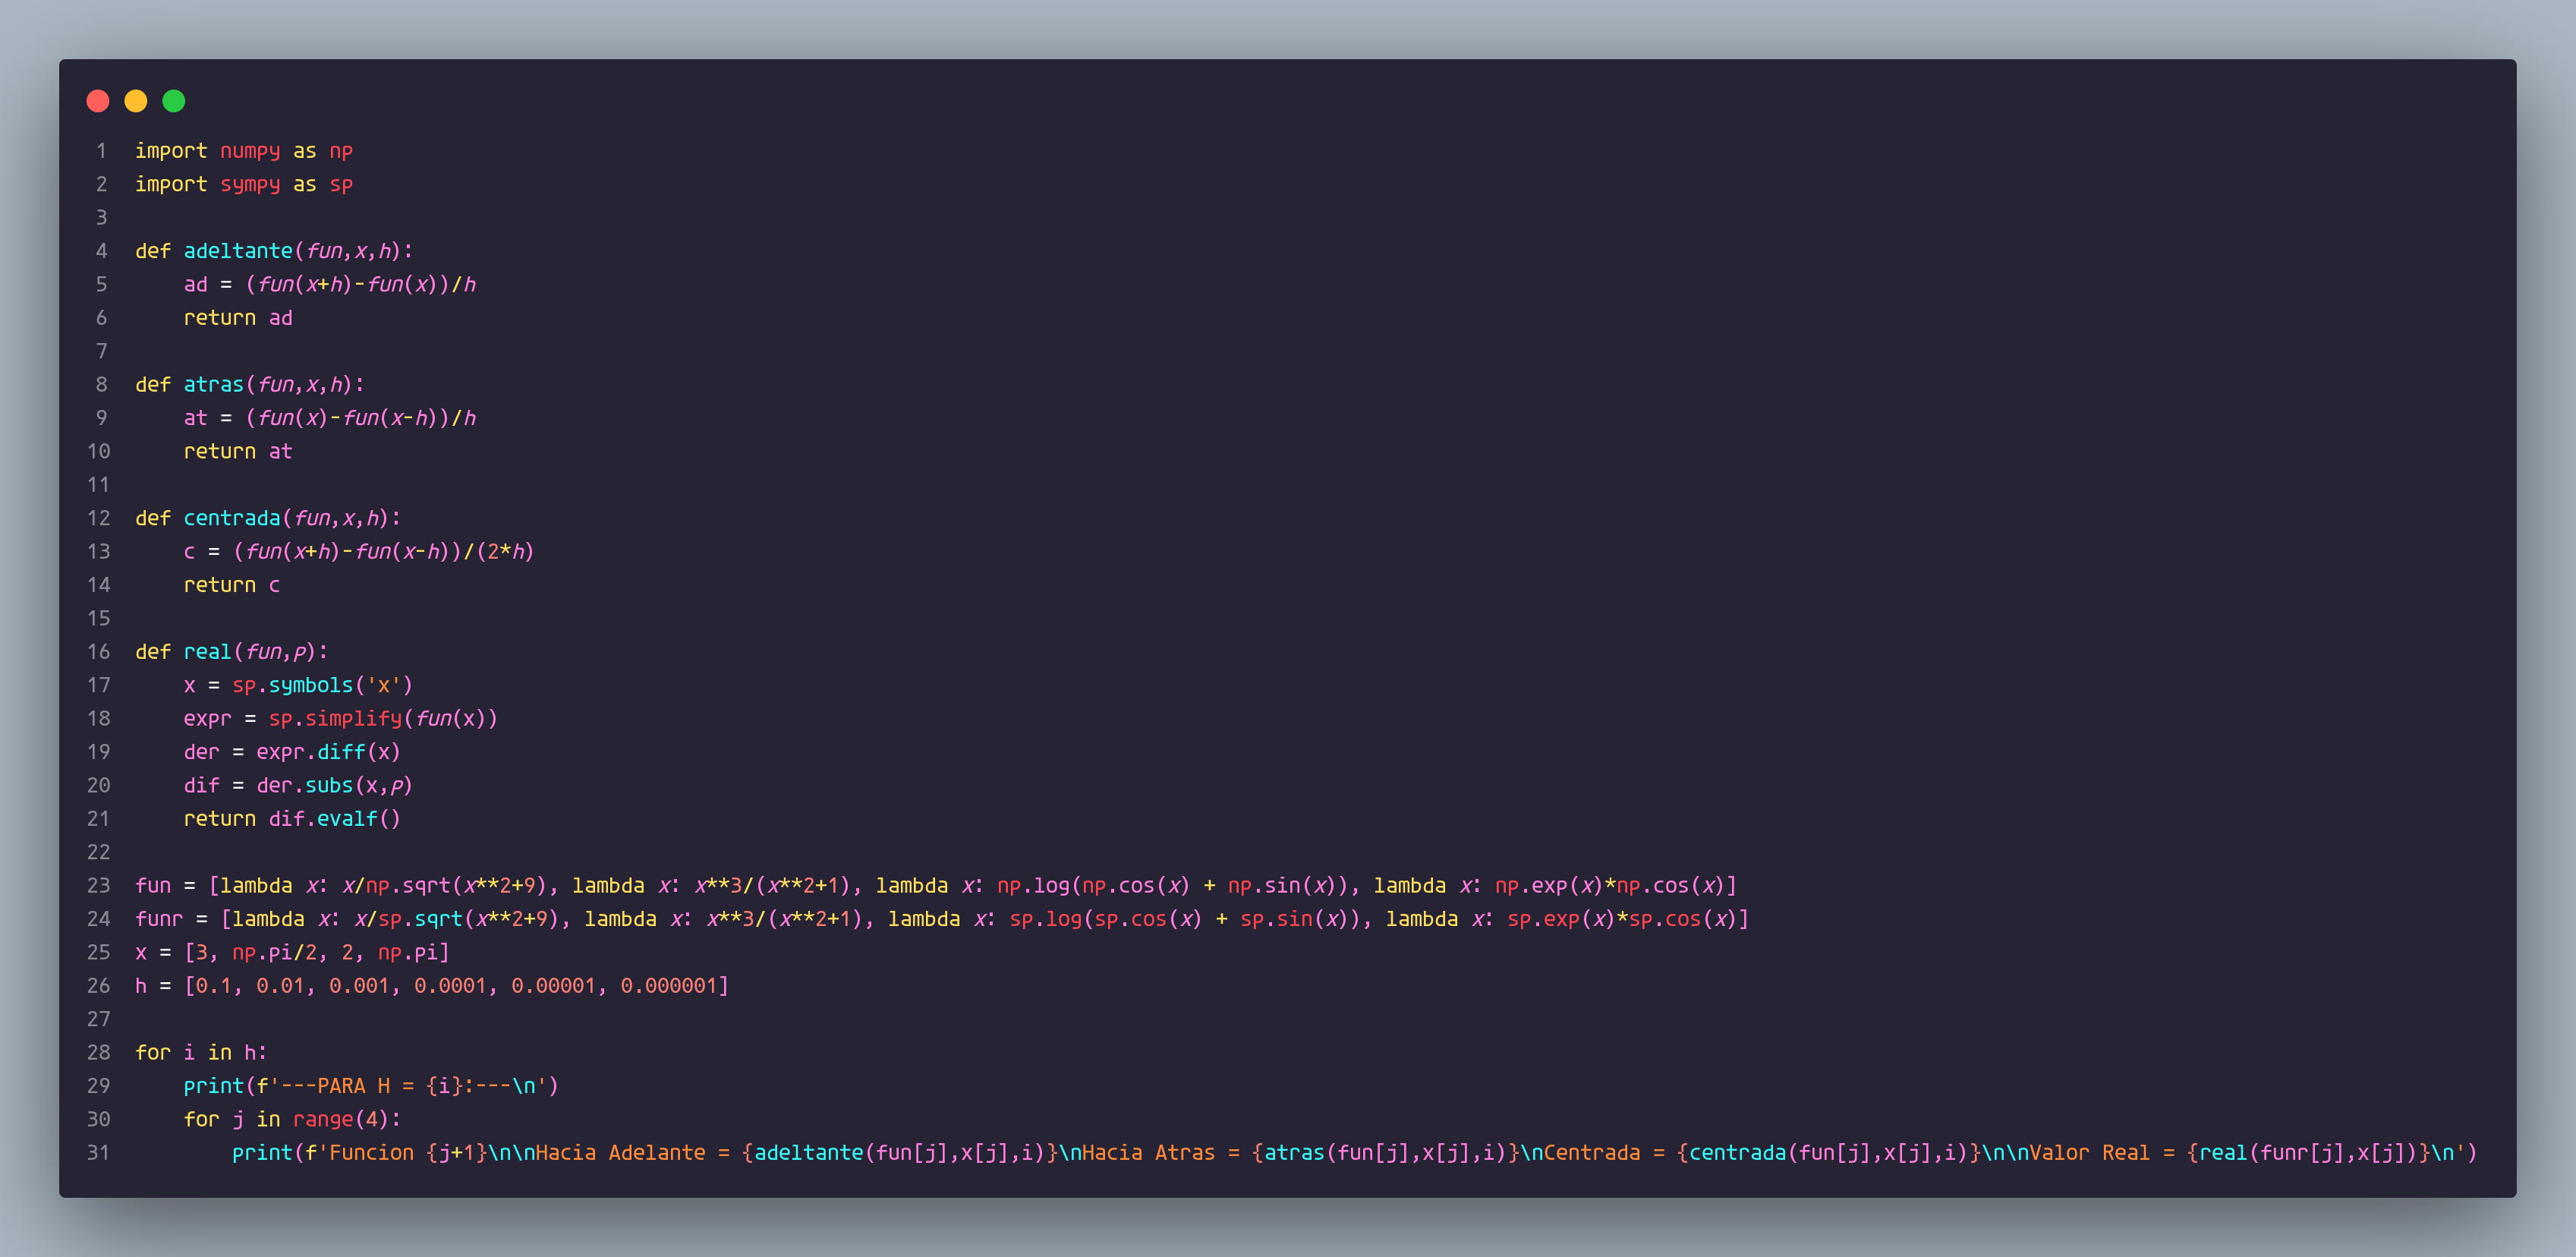
\includegraphics[width = \textwidth, height = 9cm, keepaspectratio]{code.png}
\end{figure}

\section{Resultados}

\begin{lstlisting}
    ---PARA H = 0.1:---

Funcion 1

Hacia Adelante = 0.11495360580043301
Hacia Atras = 0.12084684339072727
Centrada = 0.11790022459558014

Valor Real = 0.117851130197758

Funcion 2

Hacia Adelante = 1.118299445471349
Hacia Atras = 1.1214750542299368
Centrada = 1.119887249850643

Valor Real = 1.12000000000000

Funcion 3

Hacia Adelante = -1.1074079831006804
Hacia Atras = -0.9060602525765957
Centrada = -1.0067341178386382

Valor Real = -1.00000000000000

Funcion 4

Hacia Adelante = -23.0596231105822
Hacia Atras = -23.067336672956564
Centrada = -23.063479891769383

Valor Real = -23.1406926327793

---PARA H = 0.01:---

Funcion 1

Hacia Adelante = 0.11755699307660628
Hacia Atras = 0.11814624940961194
Centrada = 0.1178516212431091

Valor Real = 0.117851130197758

Funcion 2

Hacia Adelante = 1.1198388920854452
Hacia Atras = 1.1201588677647978
Centrada = 1.1199988799251215

Valor Real = 1.12000000000000

Funcion 3

Hacia Adelante = -1.0100673400718947
Hacia Atras = -0.990066006596319
Centrada = -1.0000666733341068

Valor Real = -1.00000000000000

Funcion 4

Hacia Adelante = -23.139917411862143
Hacia Atras = -23.13992512542633
Centrada = -23.139921268644237

Valor Real = -23.1406926327793

---PARA H = 0.001:---

Funcion 1

Hacia Adelante = 0.11782167232532448
Hacia Atras = 0.11788059789119565
Centrada = 0.11785113510826006

Valor Real = 0.117851130197758

Funcion 2

Hacia Adelante = 1.1199839888116347
Hacia Atras = 1.1200159887878591
Centrada = 1.119999988799747

Valor Real = 1.12000000000000

Funcion 3

Hacia Adelante = -1.0010006673338605
Hacia Atras = -0.9990006660005417
Centrada = -1.000000666667201

Valor Real = -1.00000000000000

Funcion 4

Hacia Adelante = -23.14068491535437
Hacia Atras = -23.140684923070864
Centrada = -23.140684919212617

Valor Real = -23.1406926327793

---PARA H = 0.0001:---

Funcion 1

Hacia Adelante = 0.11784818396809449
Hacia Atras = 0.11785407652675772
Centrada = 0.1178511302474261

Valor Real = 0.117851130197758

Funcion 2

Hacia Adelante = 1.1199983998899654
Hacia Atras = 1.1200015998880097
Centrada = 1.1199999998889876

Valor Real = 1.12000000000000

Funcion 3

Hacia Adelante = -1.0001000066660726
Hacia Atras = -0.9999000066674841
Centrada = -1.0000000066667782

Valor Real = -1.00000000000000

Funcion 4

Hacia Adelante = -23.140692555685405
Hacia Atras = -23.140692555720932
Centrada = -23.14069255570317

Valor Real = -23.1406926327793

---PARA H = 1e-05:---

Funcion 1

Hacia Adelante = 0.11785083557924735
Hacia Atras = 0.11785142483011767
Centrada = 0.1178511302046825

Valor Real = 0.117851130197758

Funcion 2

Hacia Adelante = 1.1199998400046596
Hacia Atras = 1.1200001600153442
Centrada = 1.1200000000100019

Valor Real = 1.12000000000000

Funcion 3

Hacia Adelante = -1.0000100000680943
Hacia Atras = -0.9999900000894699
Centrada = -1.000000000078782

Valor Real = -1.00000000000000

Funcion 4

Hacia Adelante = -23.14069263178453
Hacia Atras = -23.1406926321398
Centrada = -23.140692631962164

Valor Real = -23.1406926327793

---PARA H = 1e-06:---

Funcion 1

Hacia Adelante = 0.11785110065609672
Hacia Atras = 0.11785115983098393
Centrada = 0.11785113024354033

Valor Real = 0.117851130197758

Funcion 2

Hacia Adelante = 1.1199999840894037
Hacia Atras = 1.1200000160638268
Centrada = 1.1200000000766153

Valor Real = 1.12000000000000

Funcion 3

Hacia Adelante = -1.0000009998519945
Hacia Atras = -0.9999989998741164
Centrada = -0.9999999998630555

Valor Real = -1.00000000000000

Funcion 4

Hacia Adelante = -23.140692633205617
Hacia Atras = -23.14069263675833
Centrada = -23.140692634981974

Valor Real = -23.1406926327793
\end{lstlisting}

\end{document}